\section{Arrivée sur la plateforme}
\label{sec:arrivee}

La page d’accueil est une page essentielle de la plateforme. Elle doit être claire et précise car elle présente à l’utilisateur le site web.
Lorsque l’utilisateur arrive sur la plateforme, il peut directement accéder à diverses fonctionnalités. Il peut ainsi effectuer une recherche dans la base (articles, journaux, revue de presse), se connecter sur son compte utilisateur et/ou accéder à son espace utilisateur, et enfin en page d'accueil lui sont proposés des lectures tels que les revues de presse les plus récentes, les plus consultés ou les articles les plus vus.

\subsection{La recherche dans la base}
\label{sec:arrivee_recherche}
L'utilisateur peut, directement sur la page d'accueil, lancer une recherche d'un document. Il peut chercher des journaux, des articles ou des revues de presse. Respectivement, la recherche s'effectuera sur le titre des documents recherchés. Lancer la recherche emmènera l'utilisateur sur une page avec les résultats de la recherche, et la possibilité de réaliser une recherche avec de plus nombreux filtres (voir partie Recherche de documents).

\subsection{La proposition d’articles}
\label{sec:arrivee_article}
Une fonctionnalité intéressante pour l'utilisateur que nous allons développer pour la page d'accueil est, à l'instar de sites populaires comme Youtube, de proposer des lectures qui pourraient être intéressantes. On proposera ainsi à l'utilisateur de consulter directement les articles les plus vus, mais aussi les dernières revues de presse créées ou modifiées ainsi que les plus populaires. En cliquant sur un article, il sera redirigé vers la page de visualisation de celui-ci (voir partie Consultation de documents). En cliquant sur une revue de presse, il accèdera à la page de celle-ci (voir partie Revues de presse).

\subsection{Création/connexion à un compte utilisateur}
\label{sec:arrivee_utilisateur}
L’utilisateur peut, à partir de la page d'accueil, créer un compte ou se connecter à son compte utilisateur, pour par la suite accéder à son profil (voir partie Profil utilisateur).

    \begin{figure}[H]
        \centering
        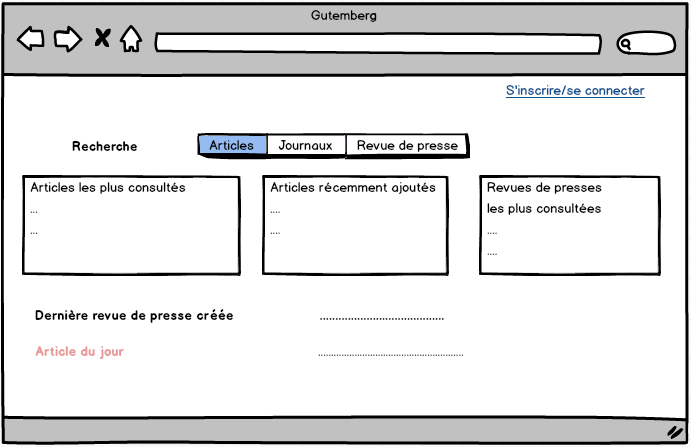
\includegraphics[width=\textwidth]{figures/Accueil.png}
            \caption{Page d'accueil de la plateforme}
            \label{fig:accueil}
    \end{figure}